\documentclass[12pt]{article}

\usepackage{hyperref}
\usepackage{amssymb}
\usepackage{amsmath}
\usepackage{epsfig, graphics}
\usepackage{latexsym}
\usepackage{fullpage}
\usepackage[parfill]{parskip}
%\usepackage{mysymbols}
\usepackage[tight]{subfigure}
\usepackage{hyperref}
\usepackage{amsmath,amssymb,enumerate,comment}
\usepackage{graphicx}

\newcommand{\figref}[1]{Fig.~\ref{#1}}

\title{10725/36725 Optimization \\Homework 1\\
{\small Due September 20, 2012 at beginning of class} \\
{Subhodeep Moitra(subhodee@andrew)}
}
\date{}

\begin{document}

\maketitle

%%%%%%%%%%%%%%%%%%%%%%%%%%%%%%%%%%%%%%%%%%%%%%%%%%%%%%%%%%%%%%%%%
%%%%%%%%%%%%%%%%%%%%%%%%%%%%%%%%%%%%%%%%%%%%%%%%%%%%%%%%%%%%%%%%%

\newpage
\clearpage

\section{Convexity (Kevin)}

\subsection{Sets}

Let $A\subseteq\mathbb{R}^n$ be a closed set with non-empty interior that has a supporting hyperplane at every point on its boundary.
\begin{enumerate}[(a)]
\item $[$4 pts$]$ 
Show that $A$ is convex.
\end{enumerate}

\vspace{.25cm}

\noindent Let $X,Y\subseteq\mathbb{R}^n$ be disjoint convex sets, let $\{x \mid a^Tx + b = 0\}$ be a separating hyperplane and let $f(x) = Cx + d$ be a function, where $C\in\mathbb{R}^{m\times n},d\in\mathbb{R}^m$.
\begin{enumerate}[(b)]
\item
$[$3 pts$]$ Given that the sets $f(X)$ and $f(Y)$ are disjoint, find a hyperplane, $\{ y \mid \alpha^Ty + \beta = 0 \}$, that separates $f(X)$ and $f(Y)$.
\end{enumerate}
Here, $f(A) = \{ y \mid y = f(x), x\in A\}$.

\subsection{Voronoi Decomposition}

Let $a,b\in\mathbb{R}^n$ such that $a\ne b$.
\begin{enumerate}[(a)]
\item
$[$2 pts$]$  Show that the set $\{ x \mid \Vert x-a \Vert_2 \le \Vert x-b \Vert_2\}$ is a halfspace.
\end{enumerate}

\vspace{.25cm} 

\noindent Let $x_1,\ldots,x_k\in\mathbb{R}^n$ and let $V_i = \{x \mid \Vert x_i-x \Vert_2 \le \Vert x_j-x \Vert_2, j\ne i \}$.
\begin{enumerate}[(b)]
\item
$[$2 pts$]$  Show that $V_1$ is a polyhedron.  That is, $V_1 = \{x \mid A_1x \le b_1\}$.
\end{enumerate}

\vspace{.25cm}

\noindent Let $P_i = \{x \mid A_ix \le b_i\}$ be disjoint polyhedra that cover $\mathbb{R}^n$.
\begin{enumerate}[(c)]
\item
 $[$3 pts$]$  Does there exist points $x_1,\ldots,x_k\in\mathbb{R}^n$ such that $V_i = P_i$ for $i = 1,\ldots,k$?  If so, provide the points, otherwise construct a counterexample.
\end{enumerate}

\subsection{Farkas' Lemma}

Let $A\in\mathbb{R}^{m\times n}, b\in\mathbb{R}^m$ such that there is some $x$ where $Ax = b$.

\begin{enumerate}[(a)]
\item
$[$6 pts$]$  Show that {\bf either} there exists $x > 0$ where $Ax = b$, {\bf or} there exists $\lambda$ such that $A^T\lambda \ge 0$, $A^T\lambda \ne 0$ and $b^T\lambda \le 0$.
\end{enumerate}
Hint: First show that $c^Tx = d$ for all $x$ such that $Ax = b$ if and only if there exists $\lambda$ such that $c= A^T\lambda, d=b^T\lambda$.

\subsection{Functions}

\begin{enumerate}[(a)]
\item
$[$3 pts$]$  Show that the function $f(x) = \left( \sum_{i=1}^n x_i^p\right)^{1/p}$ is concave on $\mathbb{R}^n_{++}$ for all $p\in(0,1)$.
\end{enumerate}
Hint: consider the log-sum-exp and geometric mean functions in Boyd.

\vspace{.5cm}

\noindent Let $G = (V,E,c,s,t)$ be an undirected graph with edge capacities $c(u,v) \ge 0$, source vertex $s$ and sink vertex $t$.  We say a vector $y\in\mathbb{R}^E$ is a valid {\em s-t-flow} if:
\begin{itemize}
\item $y(u,v) \le c(u,v), \forall (u,v)\in E$, ({\em Capacity})
\item $y(u,v) = -y(v,u), \forall (u,v)\in E$, and ({\em Skew Symmetry})
\item $\sum_{v\in V} y(u,v) = 0, \forall u\in V\setminus\{s,t\}$. ({\em Flow Conservation})
\end{itemize}
Let $f(x) = \min_y \Vert x - y \Vert$, subject to: $y$ is a valid s-t-flow.
\begin{enumerate}[(b)]
\item
$[$2 pts$]$  Show that $f(x)$ is convex.
\end{enumerate}

\newpage
\clearpage

%%%%%%%%%%%%%%%%%%%%%%%%%%%%%%%%%%%%%%%%%%%%%%%%%%%%%%%%%%%%%%%%%
%%%%%%%%%%%%%%%%%%%%%%%%%%%%%%%%%%%%%%%%%%%%%%%%%%%%%%%%%%%%%%%%%

\section{The meanest nice functions (Shiva)}

In this question, as in class, we consider optimizing `nice' functions: \begin{itemize}
\item convex on $\mathbb{R}^n$,
\item Lipschitz-continuous derivative: for some $L > 0$, $||\nabla f(x) - \nabla f(y)|| \leq L ||x - y||$ for all $x,y$.
\end{itemize}
We also restrict attention to optimization algorithms that are:
\begin{itemize}
\item first-order: the only information the algorithm gets about the function are gradients $\nabla f(x^{(k)})$. (As in class, $x^{(k)}_i$ refers to the $i$'th component of $x^{(k)}$, the $n$-dimensional vector chosen by the algorithm on the $k$'th iteration.)
\item gradient-summing: $x^{(k)}$ is a linear combination of $x^{(0)}$ and $\nabla f(x^{(0)})$ through $\nabla f(x^{(k-1)})$. 
\end{itemize}
In this question, we will prove the lower bound that was (or soon will be) stated in class.

\emph{Run any first-order, gradient summing optimization algorithm starting from any point $x^{(0)} \in \mathbb{R}^n$ for $K$ iterations, where $1 \leq K \leq \frac{1}{2}(n-1)$, yielding the last iterate $x^{(K)}$. There is a nice function $f$ such that 
$$||x^{(K)} - \bar{x}||^2 \geq \frac{1}{32} ||x^{(0)} - \bar{x}||^2,$$
$$f(x^{(K)}) - \bar{f} \geq \frac{3L||x^{(0)} - \bar{x}||^2}{32(K+1)^2},$$ 
where the minimizer and minimal cost are $\bar{x} = \textrm{argmin}_x f(x)$ and $\bar{f} = f(\bar{x})$, respectively. Thus, even upon nice functions, the convergence of rate of any such algorithm is $\Omega(1/K^2)$.}

Let's prove this lower bound together. First, assume that $x^{(0)} = 0$.
\begin{enumerate}[(a)]
\item $[$3 pts$]$ Justify this assumption. That is, if the theorem holds for $x^{(0)} = 0$, prove it still holds when $x^{(0)} \neq 0$. 
\end{enumerate}

This makes $||x^{(0)} - \bar{x}|| = ||\bar{x}||$ which will come in handy later. It also makes the initial solution `uninitialized' in every dimension. Since we required $K \leq \frac{1}{2}(n-1)$, you might have guessed there are too many dimensions for any algorithm to handle within $K$ iterations. Indeed, we will set up $f$ so that, after $k$ iterations, $x^{(k)}$ is non-zero only in its first $k$ coordinates. Since the algorithm is gradient-summing, we just need the gradients to satisfy the same condition:
\begin{align}
\forall 1 \leq k \leq K, \nabla f(x^{(k-1)}) = (\underbrace{\ldots}_{k\textrm{ numbers}}, \underbrace{\ldots}_{n-k\textrm{ zeroes}}) \label{gradzeros}
\end{align}
The lower bound on $||x^{(K)} - \bar{x}||^2$ will follow from a lower bound on the last $n-K$ coordinates of $\bar{x}$. (It would be convenient to have a formula for each coordinate of $\bar{x}$.)
The lower bound on $f(x^{(K)}) - \bar{f}$ involves a bit more thought. Imagine we have a function $g$ which agrees with $f$ at the algorithm's queries:
\begin{align}
\forall 1 \leq k \leq K, g(x^{(k)}) = f(x^{(k)}) \label{agree}
\end{align}
By definition, $\bar{g} = \textrm{argmin}_x g(x) \leq g(x^{(k)})$. By the previous two facts, 
$f(x^{(K)}) - \bar{f} \geq \bar{g} - \bar{f}$. (Now it would be convenient to have formulae for $\bar{g}$ and $\bar{f}$.) 

Rather than appealing to information theory, communication complexity, the small-set expansion conjecture, or the like, we will take a direct approach: we will explicitly construct $f$ and $g$ which satisfy (\ref{gradzeros}) and (\ref{agree}), and yield the aforementioned convenient formulae. Both functions come from the same mean family: let $f = \zeta^{(2K+1)}$ and $g = \zeta^{(K)}$, where
$$\zeta^{(k)}(x) = \frac{L}{4} \left[\frac{1}{2}\left( x_1^2 + \sum_{i=1}^{k-1}(x_i - x_{i+1})^2 + x_k^2\right) - x_1\right]$$
(The ugliness of the RHS is balanced by the typographic dubiousness of the LHS.) Convince yourself, or just take my word, that these functions are convex and continuously differentiable. Now for some math; include all your work!
\begin{enumerate}[(b)]
 \item $[$3 pts$]$ Show that $\nabla^2 \zeta^{(k)}(x) = \frac{L}{4}A^{(k)}$ for some $n \times n$ matrix $A^{(k)}$. (Write it out for a few $k$ and figure out what the block structure is.)
 \end{enumerate}
 \vspace{.25cm}
 
\begin{enumerate}[(c)]
 \item $[$3 pts$]$ Write $\nabla \zeta^{(k)}(x)$ in terms of $A^{(k)}$. Determine $\bar{x}^{(k)}_j = \textrm{argmin}_x \zeta^{(k)}(x)$ (for all coordinates $1 \leq j \leq n)$ and $\bar{\zeta}^{(k)} = \zeta^{(k)}(\bar{x}^{(k)})$ in terms of $k$, $j$, and $L$. (Just basic calculus.)
 \end{enumerate}
 \vspace{.25cm}
 
\begin{enumerate}[(d)]
 \item $[$3 pts$]$ Check that $\nabla \zeta^{(k)}$ is $L$-Lipschitz. (The definition of $L$-Lipschitz immediately suggests a way to check.)
  \end{enumerate}
 \vspace{.25cm}
 
 \begin{enumerate}[(e)]
 \item $[$3 pts$]$ Show (via induction) that $\zeta^{(k)}$ satisfies (\ref{gradzeros}).
 \end{enumerate}
 \vspace{.25cm}
  
 \begin{enumerate}[(f)]
 \item $[$3 pts$]$ Explain (quickly) why (\ref{agree}) holds.
  \end{enumerate}
 \vspace{.25cm}
 
 \begin{enumerate}[(g)]
 \item $[$4 pts$]$ Lower bound $||x^{(K)} - \bar{x}||^2$ as previously described. This involves applying the previous statements (which you should clearly mark) and some algebra (which you don't need to explain.)
  \end{enumerate}
 \vspace{.25cm}
 
 \begin{enumerate}[(h)]
 \item $[$3 pts$]$ Using $||\bar{x}^{(k)}||^2 \leq \frac{1}{3}(k+1)$, lower bound $f(x^{(K)}) - \bar{f}$. Now help yourself to a tasty square: \hfill$\square$ 
 \end{enumerate}
 \vspace{.25cm}

\newpage
\clearpage

\section{ Alternative formulations (Wooyoung)}

As discussed in class, there are often more than one way to formulate an optimization problem. In this problem, we will go through examples in which you can set up your optimization in a few alternative ways.

\subsection{Rank 1 approximation of matrices }
 
In this problem, we will set up minimizing the squared error between a given $m\times n$ matrix $A$ and a rank 1 matrix $X$. 

\begin{equation}
\text{minimize}_{\text{rank}(X)=1} ||A-X||^{2}\\
\nonumber
\end{equation}

\begin{enumerate}[(a)]
\item 
$[$1.5 pts$]$ How can you reformulate the objective function and the constraint of the above optimization by writing the space of rank 1 matrices as outer products of two vectors?
\end{enumerate}
\vspace{.25cm}

\begin{enumerate}[(b)]
\item
$[$1.5 pts$]$ One possible disadvantage of writing the space of rank 1 matrices as outer products of two vectors is degeneracy of the solutions; if a pair of vectors $\mathbf{x}$ and $\mathbf{y}$ are solutions, for any non-zero scalar $a$, $a\mathbf{x}$ and $\dfrac{1}{a}\mathbf{y}$ would also be the solutions. How would you reformulate your objective functions and constraints to avoid this degeneracy?
\end{enumerate}
\vspace{.25cm}

\begin{enumerate}[(c)]
\item 
$[$3 pts$]$ We started with one optimization variable $X$, but now we have more than one. How can you reduce the number of optimization variables in (b)? Show your work. {\it Hint:} try to show that one of the optimization variables is determined when others are fixed.
\end{enumerate}
\vspace{.25cm}

\begin{enumerate}[(d)]
\item 
$[$2 pts$]$ Reformulate the optimization problem in (c) into an equivalent minimization problem with a bi-linear objective function.
\end{enumerate}
\vspace{.25cm}

\subsection{Partial minimization of the lasso problem}

%%%%%%%%%%%%%%%
In classical setting of the lasso problem, the sparsity of solutions are enforced by $L1$-norm of the optimization variables ($\mathbf{y} \in \mathcal{R}^{d}$, $A \in \mathcal{R}^{d\times n}$, $\mathbf{x}\in \mathcal{R}^{n}$, $x_{i}$: $i$ th element of $\mathbf{x}$).
\begin{equation}
	\text{min}||\mathbf{y}-A\mathbf{x}||_{2}+\lambda ||\mathbf{x}||_{1}
	\label{lasso}
	\nonumber
\end{equation}
In this problem, we derive the partial minimization of the lasso problem.

\begin{enumerate}[(a)]
\item 
$[$2 pts$]$ How would you reformulate the optimization if we only care about the sparsity of the first $k$ elements of $\mathbf{x}$: $x_{1},x_{2},\cdots,x_{k}$. 
\end{enumerate}
\vspace{.25cm}

\begin{enumerate}[(b)]
\item 
$[$3 pts$]$ Show how you can eliminate $x_{k+1},x_{k+2},\cdots,x_{n}$ from the objective function.
\end{enumerate}
\vspace{.25cm}

\subsection{Equality constraint}

Consider an convex optimization problem with equality constraint,
\begin{eqnarray*}
&\text{minimize   } f(x)\\
&\text{subject to   } Ax = b\\
\end{eqnarray*}
Assume that the feasible set is non-empty.

\begin{enumerate}[(a)]
\item 
$[$3 pts$]$Can you remove the equality constraint by reformulating $x$ as a linear function of $z$. What conditions does the parameters of your linear function need to satisfy?
\end{enumerate}
\vspace{.25cm}

\subsection{Building a box-shape structure}
You are asked to build a box-shape structure. The area of the wall paper provided to you for the job is $A_{wall}$, and the area of the floor cannot exceed $A_{floor}$. Your picky boss even wants to control the ratio of height ($h$) to width ($w$) and also the ratio of width ($w$) to depth ($d$) of the wall structure; the ratio between $h$ and $w$ should be in the range of [$\alpha$, $\beta$], the ratio between $w$ and $d$ in [$\gamma$,$\delta$]. Your mission is to maximize the volume of the box-shape structure while satisfying all the constraints. 
\begin{enumerate}[(a)]
\item $[$2 pts$]$ Formulate your optimization problem as a maximization problem. Show your objective functions and constraints.
\end{enumerate}
\vspace{.25cm}

\begin{enumerate}[(b)]
\item $[$2 pts$]$ A geometric program is an optimization problem of the form
\begin{eqnarray*}
\text{minimize} & f_{0}(x) &\\
\text{subject to} & f_{i}(x) \leq 1, & i=1,\cdots,m\\
 & g_{i}(x) = 1, & i=1,\cdots,p\\
\end{eqnarray*}
where $g_{i}(x) = c_{i}x_{1}^{a_{1}}x_{2}^{a_{2}}\cdots x_{n}^{a_{n}}, (c_{i}>0, a_{j}\in \mathcal{R}$) and $f_{i}(x) = \sum_{k=1}^{K}c_{i,k}x_{1}^{a_{1k}}x_{2}^{a_{2}}\cdots x_{n}^{a_{nk}}, (c_{i,k}>0, a_{ik}\in \mathcal{R})$. Recently, efficient and robust algorithms have been developed to solve even large-scale geometric programs. Convert the optimization problem in (a) into a geometric programming problem.
\end{enumerate}
\vspace{.25cm}

%\begin{enumerate}[(b)]
%\item $[$2 pts$]$ Can you formulate your optimization problem into a minimization problem (not by negating the objective function in (a)) and make all your constraints to be in the form of $f(h,w,d)\leq 1$? Try to minimize the number of constraints and justify your answer.
%\end{enumerate}
%\vspace{.25cm}

\newpage
\clearpage


\section{Node by node (Kevin, Shiva)}


\begin{enumerate}[(a)]
\item $[$10 pts$]$ Derive $-\nabla\ell_T(\Theta)$.
\end{enumerate}

\begin{align*}
-\ell_T(\Theta) = -\textrm{log det}(\Theta) + \textrm{tr}(S\Theta) \\
-\nabla\ell_T(\Theta) = -\nabla \textrm{log det}(\Theta) + \nabla \textrm{tr}(S\Theta) \\
 = -\frac{\nabla \textrm{det}(\Theta)}{\textrm{det}(\Theta)} + \nabla \textrm{tr}(S\Theta)  \\
 = -(\Theta^{-1})^{T} + \nabla \textrm{tr}(S\Theta) 
 = -(\Theta^{-1})^{T} + \nabla \sum_{i=1}^{p} \sum_{k=1}^{p} {s_{ik}\Theta_{ki}} \\
 = -(\Theta^{-1})^{T} + S^T
\end{align*}

\vspace{.25cm}

\begin{enumerate}[(d)]
\item $[$9 pts$]$  Run your algorithm for $K = 5000$ iterations upon $T$ starting from the identity matrix. For each $k \in \{1,\ldots,K\}$, plot the training likelihood $\ell_T(\Theta^{(k)})$ and test likelihood $\ell_U(\Theta^{(k)})$, where $\Theta^{(k)}$ is the $k$th iterate.
\end{enumerate}

\begin{figure}[h!]
  \centering
    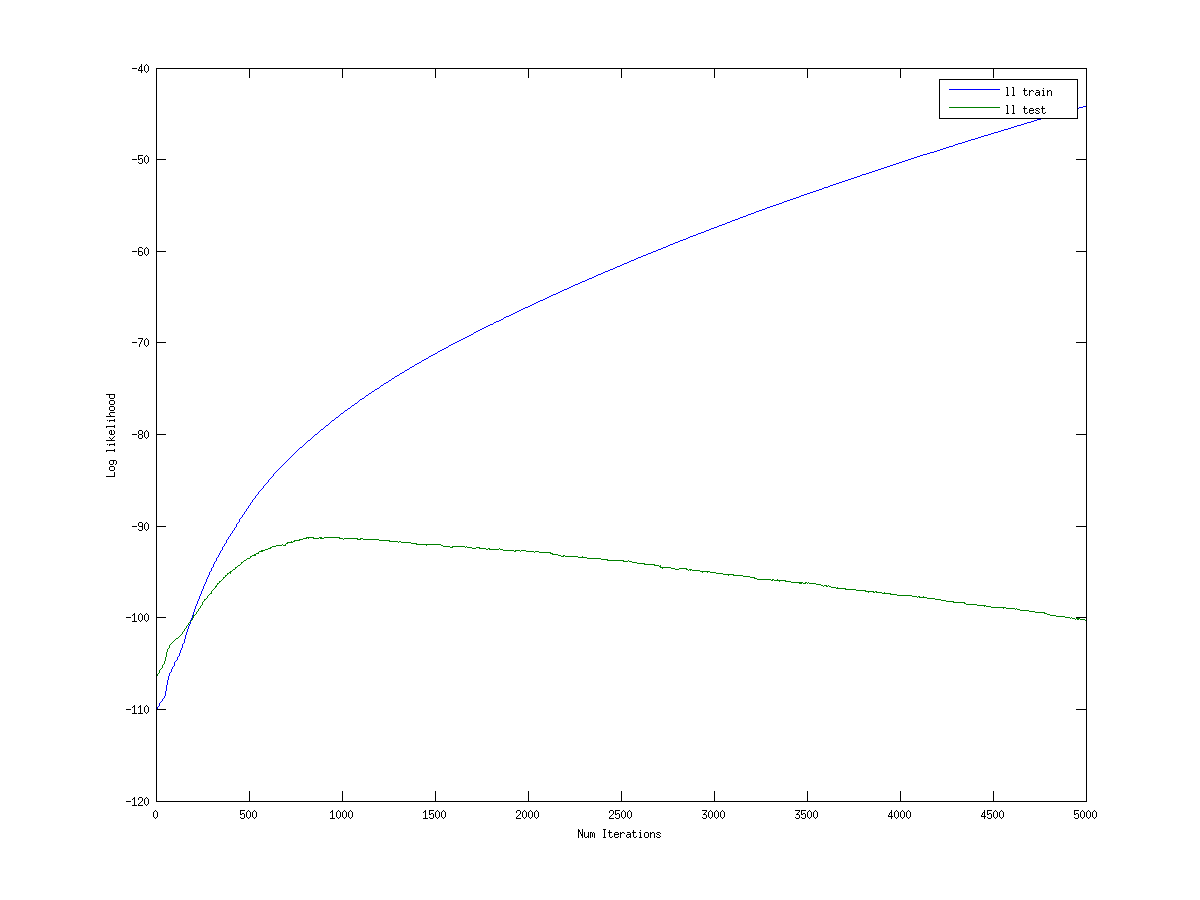
\includegraphics[width=\textwidth]{ll}
  \caption{Log likelihood Plot}
\end{figure}

\begin{enumerate}[(e)]
\item $[$8 pts$]$  Plot the matrix $\Theta^{(K)}$ in a way that emphasizes the sparsity pattern (e.g. \texttt{imagesc}).
\end{enumerate}


\begin{figure}[h!]
  \centering
    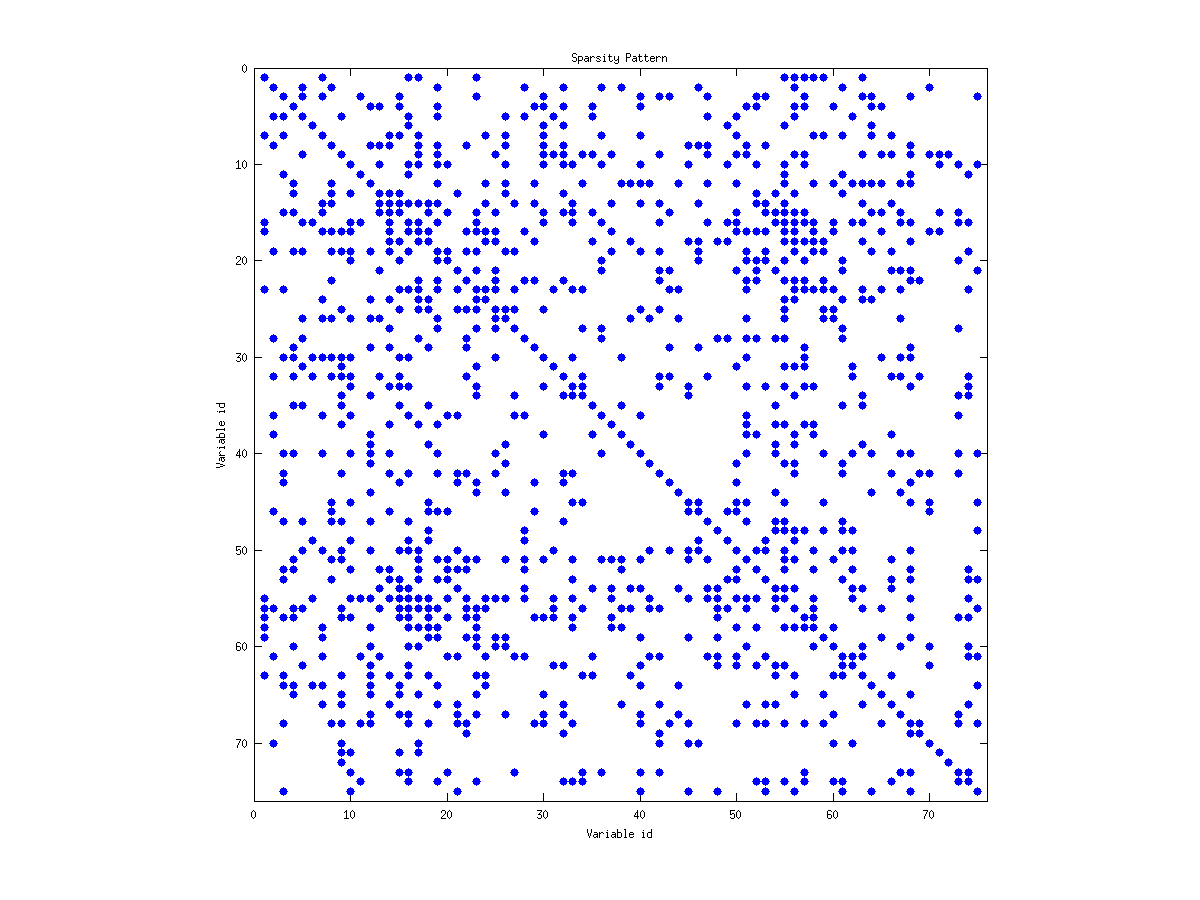
\includegraphics[width=\textwidth]{sp}
  \caption{Sparsity Visualization}
\end{figure}


\end{document}
